\documentclass[11pt,a4paper]{article}
\usepackage[margin=22mm]{geometry}
\usepackage{newtxtext,newtxmath}
\usepackage{graphicx}
\usepackage{booktabs,array}
\usepackage{adjustbox}
\usepackage{pdflscape}
\usepackage{microtype}
\usepackage{xurl}
\usepackage[hidelinks,unicode]{hyperref}
\graphicspath{{../figures/}}
\hypersetup{pdftitle={Supplementary Information: Target-specific sparse correction certificates recover stochastic language trajectories across numerical precision},pdfauthor={Lei Ke}}
\emergencystretch=2em
\setlength{\parindent}{0pt}
\setlength{\parskip}{7pt}
\setcounter{secnumdepth}{0}
\renewcommand{\thetable}{S\arabic{table}}
\setcounter{table}{1}
\title{\textbf{Supplementary Information}\\[4pt]\large Target-specific sparse correction certificates recover stochastic language trajectories across numerical precision}
\author{Lei Ke}
\date{}
\begin{document}
\maketitle


\section*{Supplementary Note 1: Official SparSamp compatibility reproduction}
\subsection{Artifact provenance.}
The reproduction used the revised SparSamp artifact from Zenodo record 15025436. The downloaded archive \texttt{Artifact \allowbreak{}new.\allowbreak{}zip} had verified MD5 \texttt{1CF080219F9F24D0C608151CEE26E99E}. The runner imported the artifact's \texttt{encode\_\allowbreak{}spar} and \texttt{decode\_\allowbreak{}spar} functions without changing their algorithm implementation. The checkpoint records SHA-256 hashes for \texttt{sparsamp.\allowbreak{}py}, \texttt{utils.\allowbreak{}py}, \texttt{get\_\allowbreak{}statistics.\allowbreak{}py} and \texttt{message.\allowbreak{}txt}, together with a fingerprint of the local GPT-2 directory.

The Basic Test generated 105 tokens, embedded 576 bits (5.486 bits/token) and recovered the complete message. The full matrix used the ten block lengths from published Table 2 and the three top-\textit{p} values from Tables 3-4. The shared block-64, top-\textit{p}=1.0 condition was executed once, giving 12 unique configurations and 1,200 configured context trials.

\subsection{Context and dependency boundary.}
The paper reports 100 IMDB contexts. The artifact \texttt{get\_\allowbreak{}statistics.\allowbreak{}py} comment also says 100, but line 49 samples 10 contexts when the context file contains more than 100. The reproduction followed the paper and selected 100 contexts once with public seed 42. Each trial used artifact seed 777, 100-200 generated tokens and the artifact message starting at offset 19.

This is a compatibility reproduction. It used Python 3.11.15, PyTorch 2.7.1+cu126, CUDA 12.6, Transformers 4.41.2 and an NVIDIA GeForce RTX 3060 Laptop GPU. Transformers 4.57.6 produced \texttt{AttributeError:\allowbreak{} \allowbreak{}'list' \allowbreak{}object \allowbreak{}has \allowbreak{}no \allowbreak{}attribute \allowbreak{}'get\_\allowbreak{}seq\_\allowbreak{}length'} at the artifact's legacy cache interface. A separate Torch 2.2.2 CUDA environment was attempted, but the upstream wheel transfer repeatedly terminated with TLS or connection-reset errors. No strict Torch 2.2.2 result is claimed.

\subsection{Outcome definitions.}
Token Ambiguity was detected by decoding each generated token sequence to public text and tokenizing it again. Completed trials with ambiguity stayed in the trial ledger but were excluded from the paper's no-ambiguity decoding and capacity denominators. A trial that reached the 200-token ceiling before completing an integer message block was recorded as budget exhausted, matching the artifact's statement that this is not an embedding error.

Embedding rate was aggregated as total encoded bits divided by total generated tokens. Entropy utilization was total encoded bits divided by total model entropy. The core reproduction gate required exact decoding for every completed no-ambiguity trial and no more than 5\% relative error for each published Table 2 utilization value and the Table 4 SparSamp embedding-rate and utilization values. Confidence intervals used 10,000 context bootstrap resamples with public seed 20260721. Timing was descriptive and had no acceptance threshold because the GPU differed from the paper.

\subsection{Results.}
The matrix completed 1,193 of 1,200 configured trials. Three block-512 trials and four block-1023 trials exhausted the 200-token budget. Among completed trials, 347 had Token Ambiguity and 846 were eligible for the no-ambiguity analysis. All 846 eligible trials decoded exactly. All 16 capacity comparisons passed the 5\% relative-error gate; the maximum relative error was 4.12\% for block length 64, top-\textit{p}=1.0 embedding rate.

The Table 2 utilization curve closely followed the published trend (Supplementary Fig. 1). Observed utilization rose from 0.272 at block length 2 to 0.872 at 32 and 0.986 at 128. The block-1023 eligible aggregate was 1.000 with a context-bootstrap interval of 0.987-1.013, compared with the published value 0.995. A finite sample can produce an aggregate embedded-bits to entropy ratio slightly above one; this observation is not interpreted as exceeding expected information-theoretic capacity.

At block length 64, the observed embedding rates were 3.672, 5.032 and 5.734 bits/token for top-\textit{p}=0.8, 0.95 and 1.0, compared with published values 3.60, 5.16 and 5.98. Corresponding utilization values were 0.963, 0.953 and 0.943, compared with 0.953, 0.949 and 0.974. These differences all remained within the prespecified 5\% relative-error tolerance.

The official reproduction therefore receives \texttt{PASS\_\allowbreak{}WITH\_\allowbreak{}LIMITATIONS}: the decoding and capacity gates passed, while seven large-block trials exceeded the fixed generation budget and the software environment was compatible rather than strict. Absolute speed is not used to support artifact fidelity.

\section*{Supplementary Table 1}
The complete machine-readable table is provided in \texttt{source\_\allowbreak{}data/\allowbreak{}supplementary\_\allowbreak{}table\_\allowbreak{}s1\_\allowbreak{}official.\allowbreak{}csv}. It reports configured completion, budget exhaustion, Token Ambiguity, eligible decoding, embedding rate, utilization with bootstrap interval, sampling time, time ratio, generation speed and embedding/decoding speed for every configuration.

\section*{Reproducibility boundary}
The raw 1,200-trial checkpoint is excluded from Git with other model outputs. Every trial was written atomically, and resuming required an exact configuration match. The tracked analysis file stores the raw-checkpoint SHA-256, software environment, bootstrap settings, configuration summaries and acceptance details. Reproduction of the exact timing numbers requires the recorded GPU and software stack; reproduction of the capacity comparison requires the unchanged artifact code, the recorded contexts and the local GPT-2 checkpoint identified by the stored fingerprint.

\section*{Supplementary Note 2: Mechanism and trust-boundary comparison}
The main study concerns target-specific token-trajectory replay, not secret-message transmission. Table S2 separates adjacent mechanisms by objective and state assumptions so that the SparSamp compatibility result is not treated as inherited evidence for SPRC novelty.

\clearpage
\begin{landscape}
\begin{table}
\centering
\caption{Mechanism and trust-boundary comparison.}
\label{tab:s2}
\scriptsize
\setlength{\tabcolsep}{3.5pt}
\renewcommand{\arraystretch}{1.18}
\resizebox{\linewidth}{!}{%
\begin{tabular}{lccccc}
\toprule
\textbf{Mechanism} & \textbf{Primary objective} & \textbf{Distribution relationship} & \textbf{Recipient state} & \textbf{Exact selected-path replay} & \textbf{Tokenization layer} \\
\midrule
Public seed only & Re-run stochastic inference & Uses the target implementation's local distribution & Model, prompt, configuration and seed & No; 5/20 on the frozen seed-0 subset & Shared tokenizer only \\
Full token trace & Store the selected path & Does not regenerate a distribution & Complete token sequence plus tokenizer & Yes, target-independent & Shared tokenizer only \\
SPRC & Repair a known target's seeded path & Quantized top-\textit{k} integer contract; truncation and quantization disclosed & Reference bundle, target identity and sparse corrections & Yes, conditional on the constructed target & Shared tokenizer only \\
Unquantized top-two delta & Isolate the probability-contract contribution & Same HMAC fraction and top-two support without bins or integer mass & Reference bundle, target identity and sparse corrections & Yes, conditional on the constructed target & Shared tokenizer only \\
Unquantized top-16-cap delta & Probe wider positive support & Up to 16 positive-probability BF16 candidates; one support shortfall observed & Reference bundle, target identity and sparse corrections & Yes, conditional on the constructed target & Shared tokenizer only \\
Fixed block repair & Repair every block containing a disagreement & Same contract as SPRC & Reference bundle, target identity and dirty reference blocks & Yes, conditional on the constructed target & Shared tokenizer only \\
SparSamp \cite{ref3} & Provably secure message embedding under its threat model & Probability-partition sampling claim & Model/context plus message-decoding state & Not its primary objective & Token Ambiguity is a separate condition \\
Range coding \cite{ref4} & Efficient secure linguistic coding & Range partition over next-token probabilities & Synchronized coder state & Not its primary objective & Shared tokenization assumed \\
List decoding \cite{ref7} & Improve PSS recovery/capacity trade-offs & Candidate-list coding & Decoder list/search state & Not evaluated here & Shared tokenization assumed \\
Dyadic approximation \cite{ref8} & Approximate LLM output laws with dyadic codes & Explicit rate-distribution approximation objective & Dyadic code specification & Not evaluated here & Shared tokenization assumed \\
ReTokSync \cite{ref9} & Recover synchronization after text re-tokenization & Orthogonal to probability replay & Public text and synchronization layer & Not evaluated here & Explicitly addresses tokenization \\
\bottomrule
\end{tabular}%
}
\end{table}
\end{landscape}
\clearpage
SPRC is therefore best interpreted as a target-conditioned sparse delta format coupled to a canonical integer sampler. Its current evidence supports smaller records than fixed block repair and the matched unquantized variants on one frozen bundle. The top-two comparison isolates a small contract advantage; the top-16-cap result shows that wider unquantized support sharply increases corrections in this target stack. These data do not establish global optimality, replay security or text-channel synchronization.

\clearpage
\section*{Supplementary Figure 1}
\begin{center}
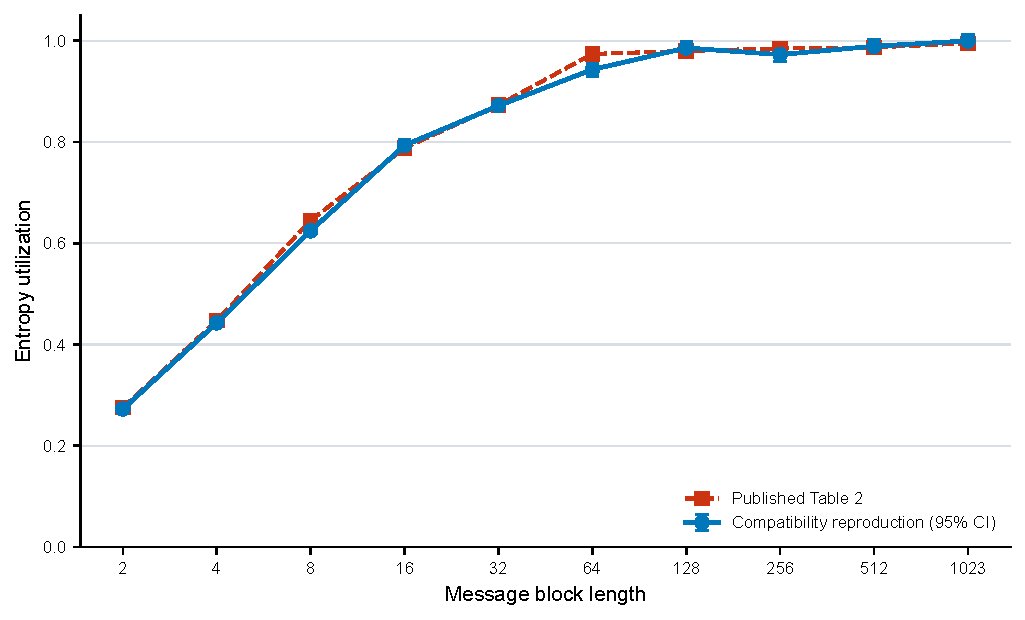
\includegraphics[width=0.96\textwidth,height=0.70\textheight,keepaspectratio]{supplementary_figure_s1_official.pdf}
\end{center}
\noindent\textbf{Supplementary Figure 1 | }Official SparSamp Table 2 compatibility reproduction. Published entropy-utilization values and the local compatibility reproduction across message block lengths 2-1023 at top-\textit{p}=1.0. Error bars show 95\% intervals from 10,000 context bootstrap resamples. The 512 and 1023 configurations contained three and four budget-exhausted trials, respectively. These trials are retained in the configured-trial count and have no capacity value.

\begin{thebibliography}{99}
\bibitem{ref1} Yuan, J. \textit{et al.} Understanding and mitigating numerical sources of nondeterminism in LLM inference. \textit{arXiv} 2506.09501 (2025).
\bibitem{ref2} Karvonen, A. \textit{et al.} DiFR: inference verification despite nondeterminism. \textit{arXiv} 2511.20621 (2025).
\bibitem{ref3} Wang, Y. \textit{et al.} SparSamp: efficient provably secure steganography based on sparse sampling. In \textit{34th USENIX Security Symposium} 6817-6835 (USENIX Association, 2025).
\bibitem{ref4} Yan, R. \& Murawaki, Y. Efficient provably secure linguistic steganography via range coding. In \textit{Proceedings of the 64th Annual Meeting of the Association for Computational Linguistics} 890-907 (Association for Computational Linguistics, 2026). \url{https://doi.org/10.18653/v1/2026.acl-long.39}.
\bibitem{ref5} Cao, W., Wang, Y. \& Hu, D. Breaking the "provable security": detecting finite-precision artifacts in LLM-based steganography via low-probability vanishing. In \textit{Findings of the Association for Computational Linguistics: ACL 2026} 20262-20274 (Association for Computational Linguistics, 2026). \url{https://doi.org/10.18653/v1/2026.findings-acl.1013}.
\bibitem{ref6} Qwen Team. Qwen2.5 technical report. \textit{arXiv} 2412.15115 (2024).
\bibitem{ref7} Pang, K. \& Bai, M. Provably secure steganography based on list decoding. \textit{arXiv} 2604.21394 (2026).
\bibitem{ref8} Bar-Lev, D., Farnoud, F. \& Gabrys, R. An additive approximation scheme for generating dyadic codings for the outputs of an LLM. \textit{arXiv} 2605.05837 (2026).
\bibitem{ref9} Wang, Y. \textit{et al.} ReTokSync: self-synchronizing tokenization disambiguation for generative linguistic steganography. \textit{arXiv} 2604.25486 (2026).
\end{thebibliography}

\end{document}
